\documentclass[a4paper,10pt]{article}

\usepackage{subfig}
\usepackage{float}
\usepackage{graphicx}
\usepackage{verbatim}
\usepackage{amsthm}

\newtheorem{defn}{Definition}
\newtheorem{prop}{Proposition}
\newtheorem{theorem}{Theorem}

%opening
\title{Degree-dependent Social Network Models}
\author{Sam Magura, Vitchyr Pong}

\begin{document}

\maketitle

\section{Introduction}

%Here we present two similar dynamic network processes that exhibit drastically different macroscopic behavior. In an iteration, we choose a node $v_0$ and break one of its incident edges.. Then, for a node $v'$ that is not adjacent to $v_0$ we add a new edge $\{v_0, v'\}$. This behavior reflects real social behavior; relationships with popular, well-connected people are potentially more valuble than relationships with less well-connected people. The model takes a parameter $I$ --- a measure of \emph{intolerance} toward unpopular people --- that determines the extent to which the degrees of adjacent nodes affect the breaking probabilities. We predicted that changing $I$ would make the model behave differently, but our simulations showed no relationship between $I$ and the model's macroscopic behavior.

\section{Model Definition}

The process operates on a graph $G = (V, E)$.

\paragraph{Definitions}
\begin{itemize}
 \item A vertex $v \in V$ is a member of the set $\mathbf{V_1}$ if and only if $0 < deg(v) < |V| - 1$.
 \item A vertex $v \in V$ is a member of the set $\mathbf{V_{out}(v_0)}$ if and only if $v \neq v_0$ and $\{v, v_0\} \notin E$. 
 \item A vertex $v \in V$ is a member of the set $\mathbf{V_{in}(v_0)}$ if and only if $\{v, v_0\} \in E$. 
\end{itemize}

\paragraph{Outline} An iteration consists of the following steps. The specifics of the breaking choice and the rewiring choice are defined separately for each of the two models.

\begin{enumerate}
 \item Choose a vertex $v_0$ randomly from $V_1$. 
 \item \emph{The breaking choice.} Choose a vertex $v^* \in V_{in}(v_0)$. 
 \item \emph{The rewiring choice.} Choose a vertex $v' \in V_{out}(v_0)$.
 \item Remove the edge $\{v_0, v^*\}$ from the graph.
 \item Add an edge $\{v_0, v'\}$ to the graph.

\end{enumerate}

Performing these steps will always be possible, provided $|V_1| > 0$. Otherwise, a $v_0$ could not be selected. Because $v_0$ is in $V_1$, it has at least one incident edge. This edge may be chosen in the breaking choice and broken. On other hand, because $v_0$ is in $V_1$, there also exists at least one vertex $v' \in V$ that $v_0$ is not adjacent to. This vertex may be chosen in the rewiring choice. 

\subsection{Breaking-function Model}

Define the behavior of the \emph{breaking-function model} as follows.

\begin{description}
 \item[The breaking choice]

 Let the chance that some vertex $v \in V_{in}(v_0)$ is chosen be proportional to

 \begin{equation}
\label{eqn:breaking-function}
 B(v) = \frac{I}{deg(v)} + \frac{1 - I}{\overline{deg}}
 \end{equation}

where $\overline{deg}$ is the mean degree of the vertices in the graph. $I$ is in the range $[0, 1]$. This is the \emph{breaking function}. We chose to use the mean degree here because the values of the two terms of the breaking function should be balanced. Additionally, the second term should be independent of $v_0$ and $v$.

 \item[The rewiring choice] Randomly select a $v'$ from $V_{out}(v_0)$.
\end{description}

\subsection{Rewiring-function Model}

Define the behavior of the \emph{rewiring-function model} as follows.

\begin{description}
 \item[The breaking choice] Let each vertex $v$ adjacent to $v_0$ have the same chance of being chosen.

 \item[The rewiring choice] For a vertex $v \in V_{out}(v_0)$, let the chance that $v$ is selected be proportional to

 \begin{equation}
\label{eqn:rewiring-function}
 R(v) = I \cdot deg(v) + (1 - I) \cdot \overline{deg}
 \end{equation}

where $\overline{deg}$ is the mean degree of the vertices in the graph. This is the \emph{rewiring function}. Unlike in the breaking function, $I$ is in the range $[0, 1)$. We do not allow $I$ to equal 1 in order to avoid a potential problem. If $I = 1$, and each vertex in $v \in V_{out}(v_0)$ has a degree of 0, then $R(v) = 0$ for each $v$, and the rewiring choice cannot be made. 
  
\paragraph{} The mean degree is used in the rewiring function because the values of the two terms should be balanced. Additionally, the second term should be independent of $v_0$ and $v^*$.

\end{description}

\section{Transition Probabilities}

\subsection{Markov Chain Definition}
Both models are Markov Chains. That is, the probability that the current state will change from $G$ to $H$ is dependent only on $G$ and $H$, not on which states were previously visited, or the number of iterations that have been performed. Thus, the transition probability from $G$ to $H$ can be written as $P(G, H)$. To begin analyzing the models as Markov Chains, we must first define what a state is.

\begin{defn}
 A graph $G = (V, E_G)$ and a graph $H = (V, E_H)$ are the same state in the Markov Chain if and only if $E_G = E_H$.
\end{defn}

This definition applies to both models. Note that, even if two graphs are isomorphic, they are not necessarily the same state; the labeling of the vertices must also be the same. Both the break-function and rewire-function models are defined such that the current state changes each iteration --- in a single iteration, one edge is removed and another, different edge is added. Thus, $P(G, G) = 0$ for any state $G$.

\subsection{Transition Condition}
We are interested in determining the probability of transitioning from a state $G$ to some other state $H$.

 \begin{center}
\begin{figure}[H]
  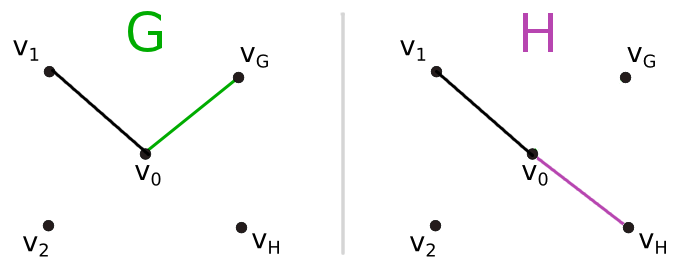
\includegraphics[height=4.0cm]{images/transition_prob.png}
  \caption{Two example states that may transition to each other.}
 \label{fig:example-states}

\end{figure}
 \end{center}

Any two states $G$ and $H$ such that $P(G, H) \neq 0$ fit the general outline given in Figure \ref{fig:example-states}. The \emph{pivot vertex} $v_P$ is the only possible $v_0$ that can result in a transition from $G$ to $H$ or $H$ to $G$. There are 0 or more vertices --- like $v_1$ --- that are adjacent to $v_P$ in both states, and there are 0 or more vertices --- like $v_2$ --- that are not adjacent to $v_P$ in either state. Finally, the \emph{the transition condition} must be met.

\begin{defn}
 States $G$ and $H$ meet the \textbf{transition condition} on pivot vertex $v_P$ if and only if $G$ has exactly one edge $\{v_P, v_G\}$ that $H$ does not, $H$ has exactly one edge $\{v_P, v_H\}$ that $G$ does not, and all other edges present in $G$ are also present in $H$. 
\end{defn}

\subsection{Breaking-function Model}

For states $G$ and $H$ that satisfy the transition condition on $v_P$, the following events must occur for a transition from $G$ to $H$ in the breaking-function model.

\begin{enumerate}
 \item In the first step, $v_P$ must be selected. Because $v_0$ is selected randomly from $V_1(G)$, the probability that $v_P$ is chosen as $v_0$ is $1 / |V_1(G)|$.
 \item The vertex $v_G$ must be chosen in the breaking choice. The chance that this occurs is $c_B(v_P \in G) \cdot B(v_G \in G)$. In order to avoid ambiguous notation later on, we choose to explicitly state which graph each function is evaluated in. The factor $c_B(v_P \in G)$ is a normalizing coefficient sufficient to normalize the breaking function values for each neighbor of $v_P$. That is,

   \begin{equation}
    c_B(v_P \in G) = \frac{1}{\sum \limits_{v \in V_{in}(v_P)} B(v \in G)}.
   \end{equation}


 \item The vertex $v_H$ must be chosen in the rewiring choice. Since the rewiring choice is made by selecting randomly from $V_{out}(v_P \in G)$, the chance that $v_H$ is chosen is $1 / |V_{out}(v_P \in G)|$.  
\end{enumerate}

All of these events must occur for a transition from $G$ to $H$. We multiply the three probabilities from the preceding list to reach the following conclusion:

\begin{theorem}
\label{thm:breaking-trans-prob}
For two states $G$ and $H$ that satisfy the transition condition on $v_P$, the transition probability from $G$ to $H$ in the breaking-function model is given by
\begin{equation}
\label{eqn:breaking-trans-prob}
P(G, H) = \frac{c_B(v_P \in G) \cdot B(v_G \in G)}{|V_1(G)| \cdot |V_{out}(v_P \in G)|}
\end{equation}
where $v_G$ is the vertex that is adjacent to $v_P$ in $G$ but not $H$.
\end{theorem}

\subsection{Rewiring-function Model}

For states $G$ and $H$ that satisfy the transition condition on $v_P$, the following events must occur for a transition from $G$ to $H$ in the rewiring-function model.

\begin{enumerate}
 \item In the first step, $v_P$ must be selected. Because $v_0$ is selected randomly from $V_1(G)$, the probability that $v_P$ is chosen as $v_0$ is $1 / |V_1(G)|$.
 \item The vertex $v_G$ must be chosen in the breaking choice. Because a vertex is selected randomly from $V_{in}(v_P \in G)$, i.e. the set of the neighbors of $v_P$,  the chance the $v_G$ is selected is $1/|V_{in}(v_P \in G)|$. Note that this probability is equal to $1 / deg(v_P \in G)$. 

 \item The vertex $v_H$ must be chosen in the rewiring choice. The chance that this occurs is $c_R(v_P \in G) \cdot R(v_H \in G)$. The factor $c_R(v_P \in G)$ is a normalizing coefficient sufficient to normalize the rewiring function values for each neighbor of $v_P$. That is,

   \begin{equation}
    c_R(v_P \in G) = \frac{1}{\sum \limits_{v \in V_{out}(v_P \in G)} R(v \in G)}.
   \end{equation}
\end{enumerate}

All of these events must occur for a transition from $G$ to $H$. We multiply the three probabilities from the preceding list to reach the following conclusion:

\begin{theorem}
\label{thm:rewiring-trans-prob}
For two states $G$ and $H$ that satisfy the transition condition on $v_P$, the transition probability from $G$ to $H$ in the rewiring-function model is given by
\begin{equation}
\label{eqn:rewiring-trans-prob}
P(G, H) = \frac{c_R(v_P \in G) \cdot R(v_H \in G)}{|V_1(G)| \cdot |V_{in}(v_P \in G)|}
\end{equation}
where $v_H$ is the vertex that is adjacent to $v_P$ in $H$ but not $G$.
\end{theorem}

Looking back on Equation \ref{eqn:breaking-trans-prob}, we see that the rewiring-function model transition probability is the same as the breaking-function transition probability, except with $c_R$ instead of $c_B$, $R$ instead of $B$, and $|V_{in}|$ instead of $|V_{out}|$.

\subsection{Verification of Results}

We implemented the two models in the Python programming language. To test our proposed transition probabilities, we created an additional Python program that implements the following procedure. The procedure can be applied to either model.

\begin{enumerate}
 \item Generate a $G(n, M)$ Erdos-Renyi graph with user-specified values for the number of vertices $n$ and the number of edges $M$. Call this initial state $G$.
 \item Make a copy $H$ of $G$. Perform a single iteration on $H$.
 \item Determine the pivot vertex $v_P$ for which $G$ and $H$ satisfy the transition condition.
 \item \emph{Measure} the transition probability $P(G, H)$ by repeating the following subroutine $L$ times. The counter $C$ is initially set to 0.

    \begin{enumerate}
      \item Make a copy $G'$ of $G$.
      \item Perform an iteration on $G'$.
      \item If $G'$ is the same state as $H$, increment the counter $C$ by 1.
    \end{enumerate}

  The observed transition probability from $G$ to $H$ is $\frac{C}{L}$.

 \item Calculate the \emph{expected} transition probability, using either Theorem \ref{thm:breaking-trans-prob} for the breaking-function model or Theorem \ref{thm:rewiring-trans-prob} for the rewiring-function model.

 \item Calculate and report the relative difference $\varepsilon$ between the observed and expected transition probabilities. To calculate relative difference between values $A$ and $B$, we use

 \begin{equation}
  \varepsilon = \frac{|A - B|}{(\frac{A + B}{2})}.
 \end{equation}

\end{enumerate}

This procedure can be used to verify our proposed transition probabilities because

\begin{equation}
 \lim_{L \to \infty} \frac{C}{L} = P(G, H).
\end{equation}

However, because only a finite number of trials $L$ is possible, some sampling error is unavoidable --- $\frac{C}{L}$ will (except in rare cases) not be exactly equal to $P(G, H)$. We can only expect the relative difference between the observed and expected transition probabilities $\varepsilon$ to have a negative correlation with the number of trials $L$. A smaller graph will typically result in smaller $\varepsilon$, because the number of states $G'$ for which a certain state $G$ can transition to increases as the numbers of vertices and edges increase. The following table shows the results of the procedure. 

\begin{table}[ht]
\centering
\subfloat[Break-function model]{
\begin{tabular}{c | c}
Trials $L$ & Relative difference $\varepsilon$ \\
\hline
 $10^3$ & 10.08\% \\
 $10^4$ & 1.35\% \\
 $10^5$ & 0.11\% \\
\end{tabular}}
\qquad
\subfloat[Rewire-function model]{
\begin{tabular}{c | c}
 Trials $L$ & Relative difference $\varepsilon$ \\
\hline
 $10^3$ & 13.68\% \\
 $10^4$ & 1.33\% \\
 $10^5$ & 0.22\% \\
\end{tabular}}
\caption{The results of several executions of the procedure on states with 4 vertices and 2 edges. An arbitrarily chosen $I$-value of $0.5$ was used. The same states $G$ and $H$ were used for each execution. The very low $\varepsilon$ values for $L = 10^5$ and the negative correlation between $\varepsilon$ and $L$ provide evidence that the expressions we derived for $P(G, H)$ are valid.}
\end{table}


\section{Equilibrium Distribution}

We can now determine the equilibrium distribution $\pi$ using the expressions we derived for the transition probabilities $P(G, H)$. If a transition from state $G$ to state $H$ is possible, a transition from state $H$ to state $G$ is also possible; because of this, we suspect both models are \emph{reversible} Markov chains. That is, that both models satisfy the \emph{detailed balance condition}:

\begin{equation}
 \pi(G) P(G, H) = \pi(H) P(H, G).
\end{equation}

We can confirm that the chains are reversible by finding the equilibrium distribution $\pi$ that satisfies the detailed balance condition for all states $G$ and $H$. Unlike in the previous section, we prove our result for both models simultaneously.

\subsection{Definitions}

\begin{defn}
Let $\delta(G, v_P)$ be the set of all states $G'$ such that $G$ and $G'$ satisfy the transition condition on $v_P$.
\end{defn}

The transition probabilities $P(G, H)$ for each model can be separated into two distinct parts: the part that depends on $H$, and the part that is independent of $H$.

\begin{defn} 
For states $G$ and $H$ that meet the transition condition on $v_P$ define $C(G, v_P)$ to be the part of the transition probability $P(G, H)$ that is indepenent $H$.
\end{defn}

\begin{itemize}
 \item For the break-function model,

\begin{equation}
 C(G, v_P) = \frac{c_B(v_P \in G)}{|V_1(G)| \cdot |V_{out}(v_P \in G)|}.
\end{equation}

 \item For the rewire-function model,

\begin{equation}
 C(G, v_P) = \frac{c_R(v_P \in G)}{|V_1(G)| \cdot |V_{in}(v_P \in G)|}.
\end{equation}

\end{itemize}

Now we consider the factor we have left out.

\begin{defn} 
For states $G$ and $H$ that meet the transition condition on $v_P$ define $f(G, H)$ to be the part of the transition probability $P(G, H)$ that does depend on $H$.
\end{defn}

\begin{itemize}
 \item For the break-function model,

\begin{equation}
 f(G, H) = B(v_G \in G).
\end{equation}
While $H$ is not explicitly mentioned in the right-hand side of this equation, recall that $v_G$ is the vertex that is adjacent to $v_P$ in $G$ but not $H$.

 \item For the rewire-function model,

\begin{equation}
 f(G, H) = R(v_H \in G).
\end{equation}

\end{itemize}

Thus, a transition probability in either model can be expressed as

\begin{equation}
 P(G, H) = C(G, v_P) \cdot f(G, H).
\end{equation}

\subsection{Restricted Case}

\begin{prop}
 The detailed balance condition, restricted such that states $G$ and $H$ meet the transition condition on a certain pivot vertex $v_P$, is satisfied by

 \begin{equation}
\label{eqn:pi-k1}
  \pi(G, v_P) = k_1 \prod \limits_{H \in \delta(G, v_P)} \frac{1}{F(G, H)}
 \end{equation}
where $k_1$ is a constant.
\end{prop}

\begin{proof}
For states $G$ and $H$ that satisfy the transition condition on $v_P$, $G$ can transition to $H$ while $H$ cannot, and $H$ can transition to $G$ while $G$ cannot. There are no other differences in the states that $G$ and $H$ can transition to. That is,

\begin{equation}
\label{eqn:deltaG}
 \delta(G, v_P) \setminus \delta(H, v_P) = \{H\}
\end{equation}
and
\begin{equation}
\label{eqn:deltaH}
 \delta(H, v_P) \setminus \delta(G, v_P) = \{G\}.
\end{equation}
Now, we rearrange the factors of the detailed balance condition. 

\begin{equation}
 \frac{\pi(G)}{\pi(H)} = \frac{P(H, G)}{P(G, H)}
\end{equation}
Substituting the equilibrium probabilities $\pi$ proposed in Equation \ref{eqn:pi-k1}, we have

\begin{equation}
 \frac{P(H, J_0) \cdot P(H, J_1) \cdot P(H, J_2) \cdots P(H, G)}
{P(G, J_0) \cdot P(G, J_1) \cdot P(G, J_2) \cdots P(G, H)} = 
\frac{P(H, G)}{P(G, H)}
\end{equation}
where $J_0$, $J_1$, $J_2$, and so on, are members of both $\delta(G, v_P)$ and $\delta(H, v_P)$. From Equations \ref{eqn:deltaG} and \ref{eqn:deltaH}, we know that the 

\begin{equation}
 \frac{P(H, G)}{P(G, H)} = \frac{P(H, G)}{P(G, H)}.
\end{equation}
Thus, the detailed balance condition holds.
\end{proof}

\subsection{General Case}

\section{Dependence on $I$}

We wrote an additional script to run the model many times with different values of $I$ to see if the behavior of the model depended on $I$ in a significant way. For each trial, the script performed a large number of iterations. It then gathered several statistics on the resultant graph: number of nodes in largest component, diameter of largest component, and number of components. We predicted that the size and diameter of the largest component would increase with $I$, while the number of components would decrease with $I$. 

\subsection{Breaking-function Model}
\begin{comment}
\begin{figure}[H]
\begin{center}
\subfloat{\includegraphics[height=4cm]}
\subfloat{\includegraphics[height=4cm]{}}
\caption{Size and diameter of the largest component, for 40 nodes, 20 edges, and 1000 iterations per trial.}
\end{center}
\end{figure} 

\begin{figure}[H]
\begin{center}
\subfloat{\includegraphics[height=4cm]{}}
\subfloat{\includegraphics[height=4cm]{}}
\caption{Number of components and 20-trial means for number of components --- using 40 nodes, 20 edges, and 1000 iterations per trial.}
\end{center}
\end{figure} 

We did not notice a substantial correlation between $I$ and the size of largest component, the diameter of the largest component, or the number of components.

In order to see why there were no correlations, we tracked the size and diameter of the largest component of the graph as iterations were performed. The following plot of size of largest component versus iteration number $i$ explains why there were no correlations. 

\begin{figure}[H]
\label{fig:gc-size-iter}
\begin{center}
\includegraphics[height=5cm]{}
\caption{How the size of the largest component changes as iterations are performed. The plot for diameter of largest component was similar.}
\end{center}
\end{figure} 

The plot shows that the breaking-function model is not stable. That is, the size of the largest component does not approach a specific value. The plot shows that, often times, over half of the graph's 20 edges are in the largest component. In an iteration where one of these edges is broken, the size of the largest component can only decrease or remain the same. With the size of the largest component ranging from 5 to 21 --- for a graph with 40 nodes and 20 edges --- the existence of a correlation between this property of the graph and $I$ seems unlikely.
\end{comment}
\subsubsection{Breaking-function Model Variations}
In attempt to get more interesting results, we tried several changes to the breaking-function model. None of the changes produced correlations between $I$ and any of the three quantities we recorded.

\begin{itemize}

 \item We tried to change the breaking function itself to increase the effect of $I$ on the breaking probabilities. For example,
 \begin{equation}
  B(v) = \frac{I^2}{deg(v^)} + \frac{(1 - I)^2}{\overline{deg}}
 \end{equation}
and
 \begin{equation}
  B(v) = \frac{sin(\frac{\pi}{4}I)}{deg(v^*)} + \frac{cos(\frac{\pi}{4}I)}{\overline{deg}}.
 \end{equation}

 \item Instead of using a breaking function, we modified the model so that $v_0$ would always break its connection with its neighbor of least degree --- and if there were multiple neighbors of least degree, chose which one to break with randomly. 

\end{itemize}
 None of these changes produced correlations.


\end{document}
